% supposed to be included by another LaTeX document

\subsection{Basic Concepts}
\qidl\ implements a set of CORBA interfaces for \codine/\GRD. These interfaces
allow access to all \GRD\ functionality as an alternative to the \codapi\ C
interface. It offers an object-oriented view of the \GRD\ system, with objects
like Master, Queue and Job. To provide a high degree of consistency and allow
an easy transition from \codapi\ to \qidl, the interfaces 
are closely related to their \codapi\ counterparts (i.e. cull lists).

This section describes the basic \qidl\ features on a more abstract and
informative level, whereas section \ref{s_user_using_qidl} applies and
describes these concepts in several examples. Section \ref{s_user_events} then
introduces the event facility of \qidl, which is used in the examples of
section \ref{s_user_using_qidl_rev}.

\subsubsection{\label{s_user_objects}The Objects}
Objects have been around in \codine\ for quite a long time, but have not been
implemented in an object oriented programming language. Instead, the
\codine\ objects were (and internally still are) represented
by their cull lists. The fields of a list element are so-to-speak the
object's attributes. Unfortunately, cull lists neither distinguish between
private and public fields, nor is there a notion of read-only attributes.
So much for encapsulation.

The operations on these cull "objects" are sparse: get, add, delete, and
modify. At least some relational database-like functionality is offered with
some sort of restriction and projection. Obviously this isn't what
object-orientation is all about.

A thorough examination of \codine's cull lists reveals the following objects,
represented here by their corresponding interfaces:

\begin{Verbatim}[fontsize=\small, frame=single]
module Codine
{
   interface Master;
   interface Queue;
   interface Job;
   interface Complex;
   interface Exechost;
   interface Checkpoint;
   interface ParallelEnvironment;
   interface UserProject;
   interface UserSet;
   interface Configuration;
   interface SchedConf;
   interface ShareTreeNode;
   interface Calendar;
};
\end{Verbatim}

The very first of these interfaces (\master) is the entry point for a \qidl\
client. There is exactly one object of this type for each \codine\ 
cell.\footnote{A \textsl{cell} is the part of the computing cluster that is
controlled by \codine.} 
Its object reference is made public and can be acquired by the client (see
section \ref{s_user_connecting}). This interface offers functions to
obtain the references of all other objects---the well-known jobs, queues,
complexes, and others. \codapi\ programmers might notice the similarities
between these interfaces and the \texttt{COD\_QUEUE\_LIST}, 
\texttt{COD\_JOB\_LIST}, and other macros from the C api.

Administration hosts, submit hosts, managers, and operators
are not represented as seperate interfaces. The simplicity of these "objects"
make this superfluous. They are handled as simple string lists.
All other objects' interfaces are embedded in a namespace called
\texttt{Codine} to avoid naming conflicts.

Once the client has acquired the desired objects, it can query all public
information about them, as well as navigate to all related objects, e.g.
from a queue to its attached complexes. Given the appropriate privileges, a
client can also create, delete, or modify objects. 

Since \codine\ is a multi-user system, an object can be deleted at any time,
either because of an explicit deletion request by an authorized user, or
naturally, e.g. by the completion of a job. So all \codine\ objects are highly
volatile---an object reference my become invalid any time. A client must
always be prepared to handle this situation. It is guaranteed, though, that
throughout the lifetime of a \emph{\codine}\ object, its corresponding CORBA
object will have the same object reference, unless the \qidl\ server is shut
down and restarted again.

\subsubsection{\label{s_user_connecting}Connecting the Server}
For a client program to interact with \qidl, it must acquire a reference to the
\master\ object, from which it can navigate to all other objects
such as queues and complexes. This reference is available via:
\begin{itemize}
\item A stringified version in
\texttt{\$CODINE\_ROOT/<cell>/common/master.ior}
\item Name service, under \texttt{/<cell>/Master} (optionally)
\item Environment variable (\texttt{\$CODINE\_MASTER\_IOR}, if set)
\end{itemize}
The safest way to connect the server is the first one, since the naming
service might crash or be manipulated otherwise, or the environment variable 
might not be set in the client process' environment. If, on the other hand, the
\texttt{\$CODINE\_ROOT} path is not accessible by the client, the other two
options are preferable.

\subsubsection{\label{s_user_authentication}Authentication}
In a standard CORBA 2.0 compliant environment, the server does not know,
where a request comes from. The IIOP layer must of course know the sender's
IP address, in order to send a reply, but it is not handed down to the
server's implementation code. The client's identity (i.e. user and group id's)
gets lost completely on the way.

This poses serious problems to \codine's access control concepts of managers,
operators, owners, and users, as well as its distinction of administration and 
submit hosts. It is
therefore necessary to provide a proprietary means of authentication, which
must be both easy to use and flexible enough to be extended in the future.
The CORBA concept of \textsl{contexts} seemds to be well suited for the
implementation of such a security framework.

CORBA contexts are a rarely used feature to send name/value pairs along with
a request. For the authentication problem, there is a context called
\texttt{cod\_auth}, whose value contains an encrypted string with some
information about the calling process. This string is usually generated by a
special library call, or granted by a trusted authority. 

All \qidl\ method signatures look like this:
\begin{Verbatim}[fontsize=\small, frame=single]
module Codine {
   interface Master {
      // ...
      QueueSeq    getQueues() context("cod_auth");
      // ...
   };
};
\end{Verbatim}
The actual value of the \texttt{cod\_auth} context is of no importance to
the user. It can contain anything from simple user identification to X.509
certificates or AFS tokens, as long as it is something that can be
decoded by \codine.

\subsubsection{\label{s_user_exceptions}Exceptions}
A client must be prepared to
handle an unexpected situation---exceptions in CORBA terms. \qidl\ defines
the following three exceptions:
\begin{Verbatim}[fontsize=\small, frame=single]
module Codine {
   // Answer thrown in case of an error
   struct Answer {
      cod_ulong   status;
      cod_string  text;
   };
   typedef sequence<Answer>   AnswerSeq;

   // Common Exceptions
   exception ObjDestroyed() {};
   exception Authentication {};
   exception Error {
      AnswerSeq   answer;
   };
};
\end{Verbatim}
\begin{description}
\item[ObjDestroyed:] This exception is thrown whenever the object that the
operation was called upon no longer exists. There is a subtle difference
between this and the standard \texttt{CORBA::INV\_OBJEREF} exception, which
means that the \emph{CORBA} object no longer exists.
\texttt{Codine::ObjDestroyed} means that the \emph{\codine}\ object no longer
exists.

\begin{figure}
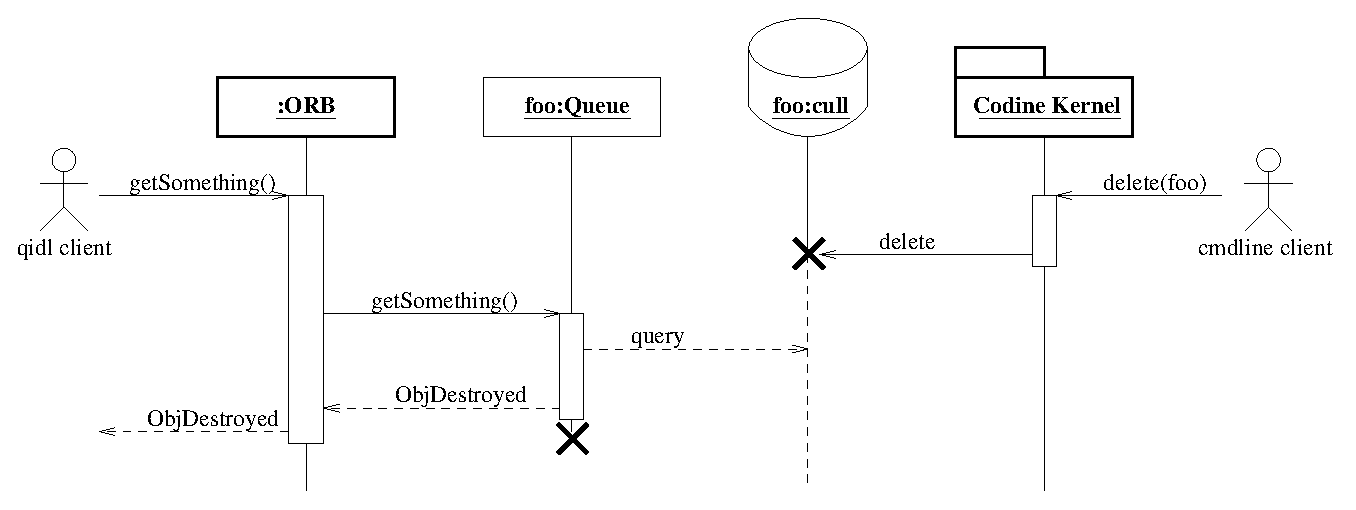
\includegraphics[width=\textwidth]{objdestroyed.eps}
\caption{\label{f_ObjDestroyed}The \texttt{Codine::ObjDestroyed} exception}
\end{figure}

Consider the situation in figure \ref{f_ObjDestroyed}. \qidl\
is a multithreaded server, so while the CORBA client's method is unmarshaled
and dispatched by the ORB (the CORBA object obviously still exists), a
command line client can delete the underlying \codine\ object. So the ORB
cannot and must not throw a \texttt{CORBA::INV\_OBJREF} exception, since
there is no reason to do so. Instead, \qidl\ notices that there is no longer
such an object and throws \texttt{Codine::ObjDestroyed}.

\item[Authentication:] As its name implies, this exception is thrown in case
of an authentication failure. Whenever there is an invalid or insufficient
\texttt{cod\_auth} context string assoiated with the operation, the client
will receive this error.

\item[Error:] Every \codapi\ call returns a so-called \textsl{answer list}.
This is a special-purpose cull list, that contains error messages and/or
warnings in case of failure, or simply a confirmation string. The
\texttt{AnswerSeq} above is the \qidl\ counterpart of the \codapi\ answer
list. The major difference between the two is that the \qidl\
\texttt{Codine::Error} exception (which contains the AnswerSeq), is only
thrown in case of an error. A \qidl\ client does not receive warnings and
confirmative messages.
\end{description}

\subsubsection{Data Retrieval and Manipulation}
After connecting to the server, considering authentication and exception
handling, a client will want to request information from \codine\ 
and add or modify data. For this purpose, \qidl\ offers a rich IDL
interface for its objects, tightly coupled with their underlying cull lists.

The first step is to retrieve references to the desired objects from the
master. The \master\ interface provides the following functions (excerpt):

\begin{Verbatim}[fontsize=\small, frame=single]
module Codine {
   interface Master : CosEventComm::PushSupplier {
      // object retrieval
      QueueSeq          getQueues() context("cod_auth");
      JobSeq            getJobs() context("cod_auth");
      ComplexSeq        getComplexes() context("cod_auth");
      ConfigurationSeq  getConfigurations() context("cod_auth");
      CalendarSeq       getCalendars() context("cod_auth");
      CheckpointSeq     getCheckpoints() context("cod_auth");
      UserSetSeq        getUserSets() context ("cod_auth");
      // ...
   };
};
\end{Verbatim}

For each class of objects, there is a corresponding \texttt{getXXXs()} method
that returns a sequence of all currently available objects of that
type.\footnote{These functions return a list of object \emph{references}, not
the object themselves, which is standard CORBA behavior.}
The client can traverse the sequence and invoke operations directly on the
contained objects, e.g. a queue (excerpt):

\begin{Verbatim}[fontsize=\small, frame=single]
module Codine {
   interface Queue : Codine::Obj {
      cod_string get_qname()
            raises(ObjDestroyed, Authentication, Error)
            context("cod_auth");
      cod_string get_qhostname()
            raises(ObjDestroyed, Authentication, Error)
            context("cod_auth");
      cod_ulong set_qhostname(in cod_string val) 
            raises(ObjDestroyed, Authentication, Error) 
            context("cod_auth");
      cod_ulong get_seq_no() 
            raises(ObjDestroyed, Authentication, Error) 
            context("cod_auth");
      cod_ulong set_seq_no(in cod_ulong val) 
            raises(ObjDestroyed, Authentication, Error) 
            context("cod_auth");
      ComplexEntrySeq get_load_thresholds() 
            raises(ObjDestroyed, Authentication, Error) 
            context("cod_auth");
      cod_ulong set_load_thresholds(in ComplexEntrySeq val) 
            raises(ObjDestroyed, Authentication, Error) 
            context("cod_auth");
      Calendar get_calendar() 
            raises(ObjDestroyed, Authentication, Error) 
            context("cod_auth");
      cod_ulong set_calendar(in Calendar val) 
            raises(ObjDestroyed, Authentication, Error) 
            context("cod_auth");
      ComplexSeq get_complex_list() 
            raises(ObjDestroyed, Authentication, Error) 
            context("cod_auth");
      cod_ulong set_complex_list(in ComplexSeq val) 
            raises(ObjDestroyed, Authentication, Error) 
            context("cod_auth");
      // ...
   };
};
\end{Verbatim}

To underline the similarity to the queue's cull list, here's an excerpt from
the \codapi\ C header file:

\begin{Verbatim}[fontsize=\small, frame=single]
LISTDEF( QU_Type )
 COD_STRING( QU_qname )        /* name of Q                    */
 COD_STRING( QU_qhostname )    /* qualified hostname           */
 COD_ULONG( QU_seq_no )        /* sequence # for use by qmon   */
 COD_LIST( QU_load_thresholds )/*   list of load alarm values  */
 COD_STRING( QU_calendar )     /* name of the calendar or NULL */
 COD_LIST( QU_complex_list )   /* user defined queue complexes */
LISTEND
\end{Verbatim}

The cull fields are translated into IDL \texttt{get\_} and \texttt{set\_}
operations. Each of these functions can raise the exceptions explained in
section \ref{s_user_exceptions}, and requires the \texttt{cod\_auth} context.
This is also the reason why \qidl\ cannot use IDL attributes, since these
don't allow user-defined exceptions and contexts. The \texttt{set\_}
functions return an integer value which is used in the context of event
handling (see section \ref{s_user_events}). Otherwise it is of no use and can
be ignored.

Apart from functions for attributes with simple data types (e.g.
\texttt{get\-\_qhostname()}, \texttt{set\_seq\_no()}), there are three other
types of functions:

\begin{itemize}
\item Functions for attributes with compound types (i.e. structs, sequences of
structs)
\item Functions for attributes with object types (i.e. object references,
sequences of object references)
\item Miscellanous and "convenience" functions
\end{itemize}

\paragraph{Functions for Attributes with Compound Types\\}
\texttt{get/set\_load\_thresholds()} are examples for this
type of function. They provide access to the queue's load alarm values,
stored in a sequence of structs of type \texttt{Codine::ComplexEntry} which
is defined as follows:

\begin{Verbatim}[fontsize=\small, frame=single]
module Codine {
   struct ComplexEntry {
      cod_string name;
      cod_string shortcut;
      cod_ulong valtype;
      cod_string stringval;
      cod_ulong relop;
      cod_ulong request;
      cod_ulong consumable;
      cod_ulong forced;
   };
   typedef sequence<ComplexEntry> ComplexEntrySeq;
};
\end{Verbatim}

Again, this structure is a direct translation of the corresponding cull list
type. But since this is only a container for a set of data and no long-lived
object controlled by the master, it is not transformed into an interface, but
only into a struct. As the CORBA standard specifies, the sequence really
\emph{contains} these data structures, not only references to them.

\paragraph{Functions for Attributes with Object Types\\}
The last four functions of the \queue\ interface concern the links of a queue
to other objects; in this case to its associated \calendar\ and \complex\
objects. These functions take or return \emph{references} or a \emph{sequence
of references} to objects managed by \master.

Note that the queue's cull list identifies its calendar only with its name
(\texttt{COD\_STRING( QU\_calendar )}), whereas in \qidl\ it is a real object
reference. In addition, there is no distinction between object reference and
struct containment in the cull, as can be seen from the
\texttt{QU\_load\_thresholds} and \texttt{QU\_complex\_list} entries; both
are of type \texttt{COD\_LIST}. \qidl\
provides a far better distinction here and reflects the true nature of the
objects' structure and interconnections.

\paragraph{Miscellanous and Convenience Functions\\}
Creation and deletion of objects fall under this category. Convenience
functions are those that would otherwise require the manipulation of certain
attributes in a certain way, just to achieve one simple goal. This
includes functions to hold or suspend a job, among others. The following two
subsections describe these in more detail.

Every retrieval or manipulation of an object's data requires a seperate COR\-BA
request. Depending on the underlying software implementation and network
structure, this can pose serious performance problems to both the client and
the master. To overcome this, every object offers functions to retrieve or
manipulate the object's state in one single method invocation. These are
defined in a common base interface from which all other interfaces except
\master\ are derived:

\begin{Verbatim}[fontsize=\small, frame=single]
module Codine {
   // Content of an object as (name,value) pairs
   struct content {
      cod_ulong   elem;
      any         value;
   };
   typedef sequence<content> contentSeq;

   // THE base class
   interface Obj {
      // opaque object state
      contentSeq  get_content() 
            context("cod_auth");
      cod_ulong   set_content(in contentSeq state) 
            context("cod_auth");
      
      oneway void destroy() context("cod_auth");
   };
};
\end{Verbatim}

The \texttt{Codine::content} structure represents exactly one field of a cull
list element. It is identified by its unique element key (\texttt{elem}), and
its value of type \texttt{CORBA::any}. The element keys are defined as
constants with the same identifier as their corresponding entries in
the cull list definitions (e.g. \texttt{QU\_qhostname}). These constants can
be found in the file \texttt{elem\_codes.idl}, a small excerpt of which is shown
here:

\begin{Verbatim}[fontsize=\small, frame=single]
module Codine {
   const unsigned long JB_job_number = 50;
   const unsigned long JB_script_file = 53;
   const unsigned long JB_script_size = 54;
   const unsigned long JB_script_ptr = 55;
   const unsigned long JB_submission_time = 57;
   const unsigned long JB_start_time = 58;
   const unsigned long JB_end_time = 59;
   const unsigned long JB_owner = 60;
   const unsigned long JB_account = 75;
   const unsigned long JB_cell = 80;
   // ...
   const unsigned long QU_qname = 250;
   const unsigned long QU_qhostname = 251;
   const unsigned long QU_priority = 261;
   const unsigned long QU_qtype = 263;
   const unsigned long QU_processors = 264;
   const unsigned long QU_job_slots = 265;
   const unsigned long QU_prolog = 267;
   // ...
   const unsigned long EH_scaling_list = 451;
   const unsigned long EH_complex_list = 452;
   const unsigned long EH_consumable_config_list = 453;
   const unsigned long EH_usage_scaling_list = 454;
   const unsigned long EH_load_list = 455;
   const unsigned long HL_name = 700;
   const unsigned long HL_value = 701;
   const unsigned long HS_name = 750;
   const unsigned long HS_value = 751;
   // ...
};

\end{Verbatim}

An object's state can be completely described by this \texttt{contentSeq}, so
per\-formance-critical applications can and should use these functions to 
interact efficiently with \codine. A similar mechanism is used for event
handling, as described in section \ref{s_user_events}.

\subsubsection{Creating and Deleting Objects}
Deleting an object is fairly simple. Every \codine\ object presented in section
\ref{s_user_objects} is derived from a common base interface,
\texttt{Codine::Obj}, as shown in the previous subsection. Recall that apart
from the state functions it also defines a \texttt{oneway void destroy()}
method to delete the object. It's usage is straightforward; the called-upon 
object won't exist anymore, unless the calling process doesn't have the
necessary privileges to dispose it (e.g. a normal user must not delete a
queue, but is allowed to cancel the jobs he or she submitted).

Creating objects is \master's responsibility. Remember that all \codine\
objects are managed by the master, so this is the canonical instance to request
new objects from. There are corresponding functions to do so:

\begin{Verbatim}[fontsize=\small, frame=single]
module Codine {
   interface Master : CosEventComm::PushSupplier {
      // ...
      Queue          newQueue(in string name)
            context("cod_auth");
      Job            newJob() 
            context("cod_auth");
      Complex        newComplex(in string name)
            context("cod_auth");
      Configuration  newConfiguration(in string hname)
            context("cod_auth");
      Calendar       newCalendar(in string name)
            context("cod_auth");
      Checkpoint     newCheckpoint(in string name)
            context ("cod_auth");
      ParallelEnvironment newParallelEnvironment (in string name)
            context ("cod_auth");
      UserSet        newUserSet(in string name)
            context ("cod_auth");
      // ...
   };
};
\end{Verbatim}

These functions return a reference to the newly created object. This
object is \emph{not} yet publicly visible to any other \codine\ client except
the one that created it, since other users should not see 
objects currently in their creation process. To permanently save an object in
the master's database and thus making it available to other users,
each object provides a corresponding \texttt{add()} function (for jobs
this is naturally called \texttt{submit()}).

\subsubsection{\label{s_user_convenience}Convenience Functions}
Convenience functions encapsulate common manipulations of object states in
easy-to-use methods. The following paragraphs show and---if 
necessary---ex\-plain
these functions for each \codine\ object. Most of them return an integer value
for use with event handling (section \ref{s_user_events}).
Note that this feature is still under development and more are functions are
being added permanently.

\paragraph{Job}
\begin{Verbatim}[fontsize=\small, frame=single]
module Codine {
   interface Job : Codine::Obj {
      cod_ulong   hold() 
            raises(ObjDestroyed, Authentication, Error)
            context("cod_auth");
      cod_ulong   suspend(boolean force)
            raises(ObjDestroyed, Authentication, Error)
            context("cod_auth");
   };
};
\end{Verbatim}

\paragraph{Master}
\begin{Verbatim}[fontsize=\small, frame=single]
module Codine {
   interface Master : CosEventComm::PushSupplier {
      // ...
      boolean registerObject(in unsigned long jid,
                             in Object obj);
      boolean unregisterObject(in unsigned long jid, 
                             in Object obj);

      oneway void shutdown() context("cod_auth");
      // ...
   };
};
\end{Verbatim}
\begin{description}
\item[{[un]}registerObject:] These functions allow a \codine\ job that
implements any type of CORBA server to register with \qidl. \codine\ 
associates the given object's reference with its job id. Clients can query
this information from \codine\ and thus use it as some sort of CORBA name
service.\footnote{This is of course not a name service as specified by
the OMG, but a mere coupling of job id's and object references.} 
The implementation of this
function sets or unsets a special context tag (\texttt{IOR}) in the given 
jobs data structure. See the \codine\ User's Manual for more information about
job contexts.

These functions are included in the \master\ interface to provide a simple way
for code suppliers to integrate their product with \codine. By using this
function, they don't need to retrieve the job list, find their corresponding
job object, and modify this job's context sequence.

\item[shutdown:] This shuts down the \qidl\ server. Use this with caution.
\end{description}

\subsection{\label{s_user_using_qidl}Using \qidl}
This section contains detailed code examples that show how to use \qidl\ as a
client. Section \ref{s_user_using_common} describes the common tasks that
each client has to perform in order to communicate with the \qidl\ server.
For brevity and to avoid repetition, these tasks will be omitted in the
following subsections, which highlight some common uses of \qidl. Note
that the presented examples were written using OOC's \textsl{ORBacus} CORBA
implementation. Some modifications might be necessary for use with other
ORBs, expecially concerning namespace/module support (\texttt{::} syntax
instead of \texttt{\_}).

\subsubsection{\label{s_user_using_common}Common Tasks}
Each \qidl\ client must obey to certain rules in order to establish and
maintain a stable connection to the \qidl\ server. These are:
\begin{enumerate}
\item Initialize the ORB
\item Acquire the server's object reference
\item Acquire a valid authentication string
\item Create a CORBA context object
\item Pass this context with all method invocations
\item \label{e_user_catch_exceptions}Always be prepared to catch an exception
\end{enumerate}
Initializing the ORB is vendor dependent and will not be explained further
here. For acquiring the server's object reference, a client can use any of
the three options described in section \ref{s_user_connecting}. We will use a
combination of all three in the following example. The authentication string
will come from a library function, and the creation of the CORBA context
object is standard CORBA 2.0 code.

\begin{Verbatim}[frame=lines, numbers=left, fontsize=\small, framerule=1mm]
// forward decls
CORBA_Object_ptr getMasterViaFile(CORBA_ORB_var& orb);
CORBA_Object_ptr getMasterViaNameService(CORBA_ORB_var& orb);
CORBA_Object_ptr getMasterViaEnv(CORBA_ORB_var& orb);

int main(int argc, char** argv) {
   try {
      CORBA_Object_var  obj;
      CORBA_ORB_var     orb;
      Codine_Master_var master;
      CORBA_any         any;
      CORBA_Context_ptr ctx;


      // initializing ORB...
      orb = CORBA_ORB_init(argc, argv);
      if(CORBA_is_nil(orb)) {
         cerr << "could not init ORB." << endl;
         return 1;
      }

      // trying to get the master's object reference
      obj = getMasterViaEnv(orb);
      if(CORBA_is_nil(obj))
         obj = getMasterViaNameService(orb);
      if(CORBA_is_nil(obj))
         obj = getMasterViaFile(orb);
      if(CORBA_is_nil(obj)) {
         cerr << "could not get master's object reference.";
         cerr << endl;
         return 1;
      }

      // narrow the object to the correct type
      master = Codine_Master::_narrow(obj);
      if(CORBA_is_nil(master)) {
         cerr << "could not narrow the object reference.";
         cerr << endl;
         return 1;
      }
      
      // create authentication context
      any <<= get_cod_auth();
      orb->get_default_context(ctx);
      ctx->set_one_value("cod_auth", any);

      // here comes the client code
      // ...
   }
   catch(CORBA_System_Exception& x) {
   }
   catch(Codine_ObjDestroyed& x) {
      cerr << "The object does no longer exist!" << endl;
   }
   catch(Codine_Error& x) {
      cerr << "Codine Error: " << endl;
      for(CORBA_ULong i=0; i<x.answer.length(); i++)
         cerr << x.answer[i].text;
   }
   catch(Codine_Authentication& x) {
      cerr << "Codine authentication problem!" << endl;
   }
   catch(...) {
      cerr << "Caught unknown exception!" << endl;
   }

   return 0;
}

CORBA_Object_ptr getMasterViaEnv(CORBA_ORB_var& orb) {
  if(getenv("CODINE_MASTER_IOR"))
    return orb->string_to_object(getenv("CODINE_MASTER_IOR"));
  else
    return CORBA_Object::_nil();
}

CORBA_Object_ptr getMasterViaNameService(CORBA_ORB_var& orb) {
   CORBA_Object_ptr obj = CORBA_Object::_nil();
   CORBA_Object_var ns_obj;
   CosNaming_NamingContext_var ns;
   CosNaming_Name_var name;

   try {
      ns_obj = orb->resolve_initial_references("NameService");
      if(CORBA_is_nil(ns_obj)) {
         cerr << "Don't have name service." << endl;
         return obj;
      }
      ns = CosNaming_NamingContext::_narrow(ns_obj);
      if(CORBA_is_nil(ns)) {
         cerr << "Not a name service." << endl;
         return obj;
      }
      name = new CosNaming_Name();
      name->length(2);
      name[0].id = CORBA_string_dup(getenv("CODINE_CELL")?
                         getenv("CODINE_CELL"):"default");
      name[0].kind = CORBA_string_dup("");
      name[1].id = CORBA_string_dup("cod_qidl");
      name[1].kind = CORBA_string_dup("");
   
      obj = ns->resolve(name);
   }
   catch(...) {
      cerr << "Problems with name service." << endl;
   }

   return obj;
}

CORBA_Object_ptr getMasterViaFile(CORBA_ORB_var& orb) {
   CORBA_Object_ptr obj = CORBA_Object::_nil();
   char ref[1024];
   char* croot = getenv("CODINE_ROOT");
   
   if (!croot) {
      cerr << "No CODINE_ROOT set." << endl;
      return obj;
   }
   string filename = croot;
   filename += "/default/common/master.ior";
   ifstream ref_file(filename.c_str());
   if(ref_file) 
      ref_file >> ref;
   ref_file.close();
   obj = orb -> string_to_object(ref);

   return obj;
}
\end{Verbatim}

Implementing the client's main routine is fairly straightforward considering
the rules mentioned above. After initializing the ORB in line 16, it tries to
retrieve the server's object reference by calling the three helper functions
(lines 22-40). In line 43, the client's authentication string (returned by
the library function \texttt{get\_cod\_auth()}) is pushed into a
\texttt{CORBA::Any} variable. The global CORBA context variable \texttt{ctx}
is initialized with the default context (line 44), and finally in line 45, the
\texttt{cod\_auth} entry is set as the context's only value. The actual
client code (not present in this example) can safely  use the \master\ object 
from this point.

All this code is encapsulated in a \texttt{try...catch} statement, according
to rule \ref{e_user_catch_exceptions} on page
\pageref{e_user_catch_exceptions}. Apart from the CORBA system exceptions and
other (unkown) exceptions, the three custom \qidl\ exceptions are handled
correctly (lines 50-65). Of course, the main program is not a good place to
seriously handle these exceptions, since no useful recovery is possible from
there. More fine-grained \texttt{try...catch} layers are necessary.

As mentioned before, the actual retrieval of the \qidl\ server's object
reference is done in three helper functions:

\begin{description}
\item[getMasterViaEnv:] The most trivial way to accomplish this task is to
read the \texttt{CODINE\_MASTER\_IOR} environment string and convert it to a
CORBA object reference with \texttt{CORBA::ORB.string\_to\_object()}.
\item[getMasterViaNameService:] This is a bit more complicated than the first
possibility. After successfully acquiring the name service object from the
ORB (lines 84-93), a naming context for the \qidl\ object is created in lines
94-100. Its reference is stored in \texttt{/<CODINE\_CELL>/cod\_qidl}.
\texttt{CODINE\_CELL} is the currently active cell (queried from the
corresponding environment variable), or the \texttt{default} cell. Line 102
then simply has to resolve the object from the name service.
\item[getMasterViaFile:] The safest way to retrieve the master object is to
read from the \texttt{\$CODINE\_ROOT/<cell>/common/master.ior} file, where
\codine\ writes the stringified object reference of the \qidl\ server. Lines
111-129 do right that, assuming the default cell as the currently active
\codine\ cell. \codine's root directory must of course be shared and 
read-accessible for the client process for this approach.
\end{description}

\subsubsection{Querying and Modifying Queue Attributes}
This subsection shows how to retrieve and modify
\begin{itemize}
\item simple attributes (i.e. those with a fundamental data type),
\item compound attributes (i.e those with a \texttt{struct} type), and
\item relations to other objects
\end{itemize}
of a queue. The example assumes that \codine\ is correctly installed and
running, there is at least one queue configured in the system, and all
initialization tasks as described in section \ref{s_user_using_common} 
have been performed successfully. No additional error and exception handling is
done here to keep the code more readable.
The code is executed inside a function which receives the \master\ object
reference and the context variable as parameters.

\begin{Verbatim}[frame=lines, numbers=left, fontsize=\small, framerule=1mm]
void query_mod_queue_attr(Codine_Master_ptr master,
                          CORBA_Context_ptr ctx) {
   // local variables
   CORBA_ULong                   i;
   Codine_QueueSeq_var           qs;
   Codine_Queue_var              q;
   
   // get the first queue from qmaster
   qs = master->getQueues(ctx);
   q = qs[0];                    // assume it exists

   // print out simple attributes
   cout << "QueueName: " << q->get_qname(ctx) << endl;
   cout << "on host  : " << q->get_qhostname(ctx) << endl;
   cout << "slots    : " << q->get_job_slots(ctx) << endl;
   
   // print out compound attributes
   Codine_ComplexEntrySeq_var lts;
   lts = q->get_load_thresholds(ctx);
   cout << "load thresholds:" << endl;
   for(i=0; i<lts->length(); i++) {
      cout << "   name: " << lts[i].name << endl;
      cout << "   valtype: " << lts[i].valtype << endl;
      cout << "   stringval: " << lts[i].stringval << endl;
      cout << "   ---------------------------------" << endl;
   }

   // print out relations to and contents of other objects
   Codine_ComplexSeq_var cs;
   cs = q->get_complex_list(ctx);
   cout << "attached complexes:" << endl;
   for(i=0; i<cs->length(); i++)
      cout << "   " << cs[i]->get_name(ctx) << endl;

   // modify slot number
   cout << endl << "Setting slots to 5...";
   q->set_job_slots(5, ctx);
   cout << "done." << endl;
   
   // delete load thresholds
   cout << "Removing any load thresholds...";
   lts->length(0);
   q->set_load_thresholds(lts, ctx);
   cout << "done." << endl;

   // checking modifications
   cout << endl << "Checking Modifications:" << endl;
   cout << "slots    : " << q->get_job_slots(ctx) << endl;
   lts = q->get_load_thresholds(ctx);
   if(lts->length() == 0)
      cout << "No load thresholds set." << endl;
   else
      cout << "Load thresholds still set!" << endl;
   
   // append a load threshold again
   cout << endl << "Appending a load threshold...";
   lts->length(1);
   lts[0].name = CORBA_string_dup("load_avg");
   lts[0].shortcut = CORBA_string_dup("");
   lts[0].valtype = 0;
   lts[0].stringval = CORBA_string_dup("175");
   lts[0].relop = 0;
   lts[0].request = 0;
   lts[0].consumable = 0;
   lts[0].forced = 0;
   q->set_load_thresholds(lts, ctx);
   cout << "done." << endl;

   // checking again
   cout << endl << "load thresholds now:" << endl;
   for(i=0; i<lts->length(); i++) {
      cout << "   name: " << lts[i].name << endl;
      cout << "   valtype: " << lts[i].valtype << endl;
      cout << "   stringval: " << lts[i].stringval << endl;
      cout << "   ---------------------------------" << endl;
   }
}
\end{Verbatim}

Lines 8-10 assign the first \codine\ queue in the list to the local variable
\texttt{q} (assuming there is at least one queue). Then, in lines 12-15,
three simple attributes are retrieved with their corresponding \texttt{get\_}
methods. Printing out compound attributes isn't much more complicated.
Querying the sequence of load thresholds (of type
\texttt{Codine::ComplexEntry}) and looping over its contents is performed in
lines 17-26. Note that the actual values of the sequence's contents are
\emph{not} retrieved with a function call, but with simple member access.

The queue's attached complexes are retrieved in line 30. This method returns
a sequence of object references to \complex es. Their names are printed out
in lines 31-33.

Changing attribute values is just as easy as reading them; calling the
\texttt{set\_} function is sufficient (lines 35-38). Lines 40-44 remove the
queue's load thresholds by setting the sequence length to zero (and thus
clearing it), and then setting the empty list as the new load threshold
sequence. Lines 46-53 simply check and display these changes.

Appending a load threshold (lines 55-67) is a bit more complicated, since a
complete \texttt{Codine::ComplexEntry} struct must be filled out correctly.
In the example, most of the fields have been zeroed, and apart from this, no
extra work is necessary. Lines 69-76 finally display this new load 
threshold value.

\subsubsection{Managing Object Relations}
In the previous example we have seen how to display a queue's attached
complexes, but we didn't change them. Modifying related objects isn't really 
complicated, and here is how to do it:

\begin{Verbatim}[frame=lines, numbers=left, fontsize=\small, framerule=1mm]
void obj_rel(Codine_Master_ptr master, CORBA_Context_ptr ctx) {
   // local variables
   Codine_QueueSeq_var     qs;
   Codine_ComplexSeq_var   cs;
   Codine_ComplexSeq_var   cplxs;
   CORBA_ULong             q;
   CORBA_ULong             c;
   char                    choice;

   // get all queues and complexes
   qs = master->getQueues(ctx);
   cplxs = master->getComplexes(ctx);

   // prompt the user
   while(true) {
      // display queues and request one
      for(q=0; q<qs->length(); q++)
         cout << q << ": " << qs[q]->get_qname(ctx) << endl;

      cout << "Which queue (" << q << " for exit): ";
      cin >> q;
      if(q >= qs->length())
         break;

      // get and display the queue's attached complexes
      cs = qs[q]->get_complex_list(ctx);
      for(c=0; c<cs->length(); c++)
         cout << "   " << c << ": " << cs[c]->get_name(ctx) << endl;

      // prompt for an action
      cout << "(A)ttach, (R)emove, (B)ack: ";
      cin >> choice;
      switch(choice) {
         // attach a complex
         case 'a':
         case 'A':
            // display all available complexes and request one
            for(c=0; c<cplxs->length(); c++) {
               cout << "   " << c << ": " 
                    << cplxs[c]->get_name(ctx) << endl;
            }
            cout << "Which complex: ";
            cin >> c;
            
            // append the chosen complex and set the new complex list
            if(c < cplxs->length()) {
               cs->append(Codine_Complex::_duplicate(cplxs[c]));
               qs[q]->set_complex_list(cs, ctx);
            }
            break;
         // remove a complex
         case 'r':
         case 'R':
            // prompt for one and remove it from the list
            cout << "Which complex: ";
            cin >> c;
            if(c < cs->length()) {
               cs->remove(c);   // ORBacus specific sequence function
               qs[q]->set_complex_list(cs, ctx);
            }
            break;
         // quit
         default:
            break;
      }
   } 
}
\end{Verbatim}

This small program interacts with the user for displaying and modifying a
queue's attached complexes. It first displays all available queues and
prompts the user to select one (lines 16-23). Then all currently attached
complexes are retrieved and printed out (lines 25-28). The user can then
choose to attach a new complex, remove an already attached complex, or go
back to the queue list. 

Lines 34-50 handle the first case: attaching a new complex. The program
therefore displays all available complexes and prompts the user to choose one
(lines 37-43). The selected complexes reference is then duplicated and
appended\footnote{\texttt{append()} is an ORBacus specific extension
to the IDL to
C++ mapping. It increases the length of the sequence and assigns the given
value to the last entry in the list.}
to the queue's complex list (line 47). Line 48 finally commits the change by
calling the \texttt{set\_complex\_list()} function.

Removing an attached complex is just as easy as adding one. Lines 54-56
prompt the user to choose one from the previously displayed list of attached
complexes and removes\footnote{Again, \texttt{remove()} is an ORBacus
specific function to delete
the specified element of a sequence. The following elements are shifted one
entry downwards.}
this in line 58, and line 59 sends the new (shortened) sequence to the \qidl\
server.

\subsubsection{Submitting a Job}
The most common task for a \codine\ user is to submit a job.
The following example provides the
basic framework including all necessary activities that you can build upon
when submitting your own jobs with \qidl. It also presents the general
two-step strategy how to add new objects to \qidl.

\begin{Verbatim}[frame=lines, numbers=left, fontsize=\small, framerule=1mm]
void submit(Codine_Master_ptr master, CORBA_Context_ptr ctx) {
   // local variables
   Codine_Job_var   job;
   Codine_PathNameSeq_var pns;
   int len;
   string script, name;
    
   // request a new job from qidl
   // this is NOT publicly accessible
   job = master->newJob(ctx);
   
   // prompt for a name and a job script
   cout << "Name: ";
   cin >> name;
   cout << "Script: ";
   cin >> script;

   // set the necessary values
   job->set_job_name(name.c_str(), ctx);
   job->set_script_file(script.c_str(), ctx);
   job->set_script_ptr(str_from_file((char*)script.c_str(),
                       &len), ctx);
   job->set_script_size(len, ctx);
   
   // set the shell list
   pns = new Codine_PathNameSeq;
   pns->length(1);
   pns[0].path = CORBA_string_dup("/bin/sh");
   pns[0].host = CORBA_string_dup("");
   job->set_shell_list(pns, ctx);

   // do actual submit
   job->submit(ctx);
}
\end{Verbatim}

Line 10 is the first important step when adding a \qidl\ object: requesting an 
object template (in this case a \job) from the server. This template is a
full-featured \qidl\ object for which you only have to fill out the desired
fields. There is one big difference, though---template objects, i.e. those
returned from a \texttt{Codine::Master.newXXX()} function, are only visible
to the calling process. No external \codine\ client (\qidl, \codapi, or
command line) will have access to this newly created object.

Back in the example, lines 12-16 ask the user for a job name and its script.
Since this example does not allow resource requests, you should enter the
name of a simple shell script, like the \texttt{sleeper.sh} script from
\texttt{<\$CODINE\_ROOT>/\-examples/\-jobs}. You must supply the fully qualified
path name of the script. No environment variables are allowed.

Lines 18-23 then set the according values of the job template object. It uses
the function \texttt{str\_from\_file()}, a helper function that reads the file
and returns a string buffer with its contents, as well as the buffer's
length. This buffer, i.e. the script files contents, is passed to \job's
\texttt{set\_script\_ptr()} function. Instead of using
\texttt{str\_from\_file()}, you could of course as well use a custom function,
as long as the necessary job attributes are set correctly.

Since \codine\ needs to know which shell to start for the job, a
\texttt{Codine::\-PathNameSeq} must be set as the job's shell list. Lines 25-30
perform this task, assuming a bourne shell for the job script.
The actual submission of the job is done in line 33, with one simple call.
This also makes the job visible to all other \codine\ users. You can check this
by issuing a \texttt{qstat -f} command in a terminal window. Your job should
appear in its output.

Note that submission directives that are specified in the job (usually
beginning with \texttt{\#\$}) are \emph{not} evaluated by this example.
Rebuilding this \texttt{qsub} functionality with \qidl\ requires some more
effort than the few lines of code above.

\subsection{\label{s_user_events}Events}
After the examples from the previous section, the following pages describe
\qidl's event mechanism in a more abstract form. Section
\ref{s_user_using_qidl_rev} will apply these concepts again in some
real-world examples.

\subsubsection{The Need for Events}
Imagine a computing cluster with several hundreds---or even thousands---of
workstations. The users---probably in the order of hundreds, too---regularly
submit jobs and monitor the cluster with custom \qidl\ clients. The first and
easiest approach for these clients is to regularly poll for data at the
\qidl\ server. That is, at regular intervals---say, 30 seconds---each of the
client programs requests several sequences of objects from the master, and
subsequently the state of each of these objects.

Remember that the retrieval of every single attribute of every single object 
requires a seperate CORBA method invocation---and thus two data packages sent
across the network; one forth and one back. It is clear, that the response
times will decrease drastically, because of both the network traffic, and the
additional overhead of marshaling and unmarshaling the requests on the
client and especially the server side.

This problem is not new and unique to \codine\ and \qidl---and neither is its
solution: Notification of clients in case of a change of an object. The
mechanism used to notify clients is the standard CORBA event service, and
following its terminology, a client is an \textsl{event consumer} and the
\qidl\ server is the \textsl{event supplier}. The client can request the
reference to the event channel from the \qidl\ server and then register as an
event consumer. The server pushes events into the channel whenever an object
is added, deleted, or changed.

This approach limits network traffic to a minimum compared to the polling
strategy described above. Furthermore, it reduces the server load since
\qidl\ does no longer need to handle thousands of CORBA requests per minute,
but instead only pushes \emph{one} event object with \emph{one} method
invocation (this time actually being the client, not the server)
into the event channel whenever this is necessary. The event service acts as a
multiplexer for the events.

\subsubsection{Event Contents}
The actual event is a structure defined in the file
\texttt{basic\_types.idl}:
\begin{Verbatim}[fontsize=\small, frame=single]
module Codine {
   // Content of an object as (name,value) pairs
   struct content {
      cod_ulong   elem;
      any         value;
   };
   typedef sequence<content> contentSeq;

   // ...

   // event handling stuff
   enum event_type {
      ev_add,
      ev_mod,
      ev_del
   };
   struct event {
      event_type  type;
      cod_ulong   obj;
      cod_string  name;
      cod_ulong   id;
      cod_ulong   count;
      Object      ref;
      contentSeq  changes;
   };
};
\end{Verbatim}
Its members are:
\begin{description}
\item[type:] Specifies (with the \texttt{event\_type} enumeration) if an
object was added, modified, or deleted.
\item[obj:] Specifies the class of the object that has changed, e.g.
\texttt{COD\_QUEUE\_LIST}, etc. These constants correspond to those from
\codapi.
\item[name:] The name by which the concerned object is identified, e.g. a
queue's name.
\item[id:] The numerical identifier by which the concerned object is
identified. Only used for job id's.
\item[count:] This is a unique value for each event. It corresponds to the
integer value returned by any of the \texttt{set\_} functions. The next
subsection explains its usage further.
\item[ref:] A reference to the concerned object.
\item[changes:] This member contains the actual changes of the object. It
consists of a sequence of name/value pairs (\texttt{Codine::content}) that
describe the state of the object. At the moment, the complete object state is
sent with every event, even if only a small portion of it changed. Expect
this behavior to change in the future.
\end{description}

\subsubsection{Getting and Handling Events}
This subsection explains the general strategy for a client to receive \qidl\
events. Basic knowledge of the CORBA Event Service Specification is
recommended, since its terminology is used throughout this and the following
subsection.

After the usual connection setup, a potential event consumer can acquire a
\texttt{CosEventChannelAdmin::ConsumerAdmin} object from the master, which in
turn acts as a \texttt{CosEventComm::PushSupplier}.
\begin{Verbatim}[fontsize=\small, frame=single]
module Codine {
   interface Master : CosEventComm::PushSupplier {
      // ...
      CosEventChannelAdmin::ConsumerAdmin  getConsumerAdmin()
                                              context("cod_auth");
      // ...
   };
};
\end{Verbatim}
This standard CORBA interface
allows a consumer to connect to the event channel, either via push or pull
mode. The pull mode is fairly simple, since the client can ask for events any
time it wants to. In the push model, the client has to set up a servant
object that can receive events any time the event channel wants to, i.e. any
time a new event has arrived. This servant object has to implement the
\texttt{CosEventComm::PushConsumer} interface. Its \texttt{push()} method is
called by the event channel whenever the \qidl\ server places a new event
into the channel.

Event handling is then up to the client, usually having a \texttt{switch}
statement for the type of event (add, mod, del), and one for the class of the
concerned object (\texttt{Codine::event.obj}). With the \texttt{name},
\texttt{id}, or \texttt{ref} members of the event structure, the client can
identify the actually concerned object, and map it to, create or
delete its local representation. The actual object state can be reproduced 
or updated with the \texttt{Codine::contentSeq} sent with the event.

Note that although the CORBA object reference of the concerned object is
contained in the event, the client should not use this reference and invoke
CORBA requests on it to retrieve its state---the potential performance
advantage of events evaporates with this approach. This reference is intended
only for \emph{really} unique object identification. Event clients should
always store a local copy of the complete state of all objects, or at least
of those of interest to them. So there is always an intermediate storage that
gets updated when events arrive, and is used by the actual client code (e.g.
a graphical user interface) to retrieve data from, as figure
\ref{f_user_ev_client} illustrates.

\begin{figure}
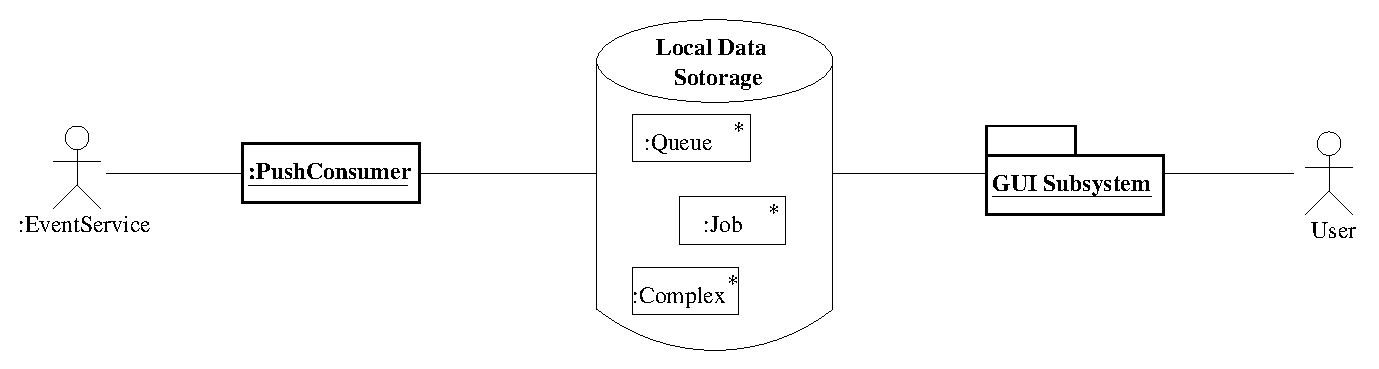
\includegraphics[width=\textwidth]{evclient.eps}
\caption{\label{f_user_ev_client}Typical logical structure of a \qidl\ event
client}
\end{figure}

\subsection{\label{s_user_using_qidl_rev}Using \qidl\ Revisited}
\subsubsection{Basic Events}
Programming with events is undoubtedly more work than programming a simple
\qidl\ client. But the gain in performance and application architecture is
worth the effort. As mentioned in the previous section, a \qidl\ event
consumer needs a local database representing the \codine\ objects, which is
updated upon the arrival of an event. It is beyond the scope of this example
to provide the complete code for this local storage or even the full client
program logic (display handling, user interaction, \dots). Furthermore will
the example only handle events for queues; other objects can be treated
similarly.

So let \texttt{MyQueue} be a C++ class that represents a \queue\ object in
the client, and \texttt{allQueues} be a global variable that stores all
queues in an STL vector class. The following example illustrates how to
register for events and handle them appropriately by updating the local data
storage. No synchronization with the actual client code---supposed to run in
a seperate thread---is done.
Let us take a look at the clients main program now. 

\begin{Verbatim}[frame=lines, numbers=left, fontsize=\small, framerule=1mm]
// forward decls
class MyQueue;
class EventClient;

// global data storage
vector<MyQueue*>   allQueues;

// the main program
int main(int argc, char** argv) {
   // initialize ORB, BOA, Context, QIDL Master, ...

   // setup event client
   EventClient* consumer = new EventClient(master);

   // start UI thread here
   // ...

   // accept events
   boa->impl_is_ready(...);

   return 0;
}
\end{Verbatim}

After the usual initialization tasks described in section 
\ref{s_user_using_common},
the main routine creates an object of type \texttt{EventClient} in line 13.
This is a custom class that does the actual event handling. After starting
one or more other threads to handle user input, the servant object is
connected to the CORBA bus by calling \texttt{impl\_is\_ready()} in line 19.
This blocks the main thread and incoming events are dispatched in the
\texttt{EventClient}'s \texttt{push()} function.

\begin{Verbatim}[frame=lines, numbers=left, fontsize=\small, framerule=1mm]
// class EventClient
class EventClient : virtual public CosEventComm_PushConsumer_skel {
   public:
      EventClient(Codine_Master_ptr master, CORBA_Context_ptr ctx);
      virtual ~EventClient {}

      virtual void push(const CORBA_Any& any);
      virtual void disconnect_push_consumer() {}
};

EventClient::EventClient(Codine_Master_ptr master,
                         CORBA_Context_ptr ctx) {
   // get consumer admin from master
   CosEventChannelAdmin_ConsumerAdmin_var     ca = 
                                 master->getConsumerAdmin(ctx);
   // get proxy push supplier from consumer admin
   CosEventChannelAdmin_ProxyPushSupplier_var pps = 
                                 ca->obtain_push_supplier();

   // connect as a push consumer
   pps->connect_push_consumer(
                  CosEventComm_PushConsumer::_duplicate(this));
}

void EventClient::push(const CORBA_Any& any) {
   // extract the event structure from the Any type
   Codine_event* ev;
   any >>= ev;

   // we're only interested in queues
   if(ev->obj != COD_QUEUE_LIST)
      return;

   // what type of event
   vector<MyQueue*>::iterator it;
   switch(ev->type) {
      case Codine_ev_add:
         // create a new queue representation from the supplied
         // contents and append it to the vector
         allQueues.push_back(new MyQueue(ev->changes));
         break;
      case Codine_ev_mod:
         // find the queue and update its state
         for(it=allQueues.begin(); it!=allQueues.end(); ++it)
            if((*it)->name() == ev->name)
               (*it)->update(ev->changes);
         break;
      case Codine_ev_del:
         // find the queue and remove it from the vector
         for(it=allQueues.begin(); it!=allQueues.end(); ++it)
            if((*it)->name() == ev->name) {
               delete *it;
               allQueues.erase(it);
            }
         break;
      default:
         break;
   }
}
\end{Verbatim}

The constructor (lines 11-23) retrieves the consumer administration interface
of the event channel from the \qidl\ master, where a proxy push supplier can
be obtained. It then connects to the channel as an event consumer in push
mode.

The \texttt{push()} method itself first extracts the \texttt{Codine::event}
structure from the delivered \texttt{Any} variable (lines 27-28). If the
concerned object is not a queue, then the event handler returns immediately,
since it is not interested in other objects (lines 30-32). The switch
statement in lines 36-58 distinguished the three event types: add, mod, and
del.

The \texttt{ev\_add} event is very easy to handle. Creating a new object from
the delivered \texttt{Codine::contentSeq} and appending it to the global data
storage is all there is to do (line 40). Both the \texttt{ev\_mod} and
\texttt{ev\_del} event handlers need to find the concerned object in the
local database (lines 44-45/50-51). If found, it is either updated with the
new object state (line 46), or deleted and removed from the global queue
vector (lines 52-53).

The actual work of maintaining the object state is of course delegated to the
\texttt{MyQueue} class. It must provide a consistent mapping of the delivered
\texttt{Codine::contentSeq} to its internal data representation---whatever
this might look like.

\subsubsection{The Event Counter}
Every \texttt{set\_} function returns an integer value. This return value is
a unique event count number that is sent with the event that was generated by
the \texttt{set\_} method. So if a client wants to be sure that it displays
the right object state at all times, especially after object modifications,
it should block and wait for the arrival of the corresponding event. The
pseudocode might look like this:

\begin{Verbatim}[fontsize=\small, frame=single]
void MyQueue::commitState() {
   count = queue_ref->set_state(myLocalState, ctx);
   blockOnConditionVariable(count);
}
\end{Verbatim}

After setting the queue's state, the local queue object blocks on a condition
variable which gets signaled when the event with number \texttt{count}
arrived. The signaling is done by the event handler, e.g. like in the
following pseudocode:

\begin{Verbatim}[fontsize=\small, frame=single]
void EventClient::push(CORBA_Any& any) {
   // ...
   switch(ev->type) {
      case Codine_ev_mod:
         // ...
         signalConditionVariable(count);
         break;
      // ...
   }
   // ...
}
\end{Verbatim}

If the incoming event modified an existing object, then the event handling
can simply signal the appropriate condition variable, thus waking up all
sleeping UI threads that were waiting for this event. These threads can then
safely update the display and be sure that the data shown is new enough to
reflect the changes made by the previous \texttt{commitState()} call.
